\chapter{The vascular network}
\label{chap:network}

The 2018 brief asked for a quantified network: nodes, branches, calibre and branch lengths. With a
validated segmentation, this goal is now within reach. pyBones~\pbValueVersion{} measures the vessel
network of a segmentation (\code{pybones quantify}, or the page's \emph{Network} tab) and writes
three files next to its labels: a summary with the nodes (\code{network.json}), one row per branch
(\code{branches.csv}) and the centreline voxels (\code{centrelines.npz}).

\section{From a mask to a network}

\paragraph{Centrelines} The vessel mask is first closed: cavities (background enclosed by vessel, a
hollow lumen of a vessel imaged as a ring) are filled, otherwise a thick vessel thins into a sheet
instead of a line. It is then thinned to one-voxel centrelines (scikit-image's 3D skeletonisation),
and each centreline voxel gets its distance to the vessel wall: the local radius.

\paragraph{Graph} Touching centreline voxels (26-neighbourhood) are linked. Where three voxels touch
each other, the longest link of the triangle is dropped, unless that would disconnect them: a
diagonal step of the centreline is not a fork. A voxel with one link is an end, with three or more a
junction (touching junction voxels form one node); runs of two-link voxels between nodes are the
branches.

\paragraph{Pruning} Skeletons of real masks are hairy. Four kinds of operation repeat until none applies,
all in micrometres: a branch from a junction to a free end shorter than \pbValueNetSpurFactor{} times the widest radius at its
junction is a bump of the surface and goes, as do isolated specks; a loop barely longer than the
circumference of its vessel is a hole or a fold of the vessel mask, not a structure: a ring from a
junction back to itself goes when shorter than the circumference, and any other loop when shorter than
\pbValueNetLoopFactor{} circumferences, by its longest branch (found with a minimum spanning tree of
the network, so that nothing is ever disconnected); two junctions joined by a branch shorter than
their radii together are one fork, merged (the branch's length is kept); a node left with two branches
joins them.

\paragraph{Ends} An end within its radius (plus \pbValueNetAnchorMargin\um) of a face of the stack or of a
burst is not a free end: the vessel goes on beyond it. Such ends are never pruned, and the branches
reaching them are flagged \emph{truncated}.

\paragraph{Measures} Each branch gets its length along the centreline, its chord, their ratio (the
tortuosity) and the radius along it (mean, median, minimum, maximum). For the whole stack: the counts
of branches, junctions and ends by kind, the total length, the length per volume (length density) and
the medians.

The three 3D steps (cavities, centrelines, distances) are interchangeable implementations behind
small interfaces, chosen in the configuration: pyBones' streaming connectivity and per-slice distance
maps, or SciPy's. Both give identical results on the sample; pyBones' are faster and use less memory,
SciPy's handle non-square pixels.

\section{Validation on a branching phantom}

The phantom of Chapter~\ref{chap:validation} draws separate vessels. For the network, its vessels can
branch: a walk may start a thinner child at its current point, and the phantom records every true
centreline segment, its radius and every bifurcation. A dedicated phantom (\pbValueNetPhantomVessels{} vessels branching up to
\pbValueNetPhantomDepth{} levels deep, same calibration) is generated afresh for this report, segmented, and its network
measured twice: on its \emph{true} mask, to test the quantification alone, and on its segmentation,
to test the whole chain (Table~\ref{tab:network-scores}). A centreline is found when it lies within
\pbValueNetTolerance\um{} of the truth; a fork is found within \pbValueNetJunctionTolerance\um{} plus the radius of
its parent vessel.

\begin{table}[ht]
  \centering
  \small
  \begin{tabular}{lrrrrrrr}
\toprule
On & Recall & Precision & Forks & Not forks & Crossings & Length (mm) & Radius ($\mu$m) \\
\midrule
True mask & 0.96 & 0.96 & 40 / 53 & 8 & 7 & 23.50 / 21.72 & $-0.67$ \\
Segmentation & 0.79 & 0.85 & 26 / 53 & 49 & 7 & 21.06 / 21.72 & $-0.82$ \\
\bottomrule
\end{tabular}

  \caption{The network of the branching phantom, measured on its true mask and on its segmentation.
    Recall: share of the true centrelines found; precision: share of the measured centrelines that are
    true. \emph{Forks}: true bifurcations found; \emph{not forks}: other measured junctions;
    \emph{crossings}: junctions where two separate vessels touch (real junctions of the mask, not
    bifurcations). Length: measured / true; radius: median offset from the true radius.}
  \label{tab:network-scores}
\end{table}

\paragraph{Lengths} On the segmentation, the total length differs from the truth by
\pbValueNetSegLengthErrorPct\,\%. It is the net of two errors in opposite directions: the thin vessels
the segmentation misses (centreline recall \pbValueNetSegRecall) shorten it, and strands doubled where
the vessel mask has holes lengthen it. Pruning the small loops removes most doubled strands, so what
remains is mostly the thin vessels missed.

\paragraph{Junctions are over-counted} Even on the true mask, \pbValueNetTrueMaskMissed{} of the \pbValueNetTrueForks{} forks are not
found (two close forks merge into one, a short side branch is pruned as a spur), and
\pbValueNetTrueMaskSpurious{} junctions are not forks. On the segmentation, only \pbValueNetSegForks{}
forks are found, and \pbValueNetSegSpurious{} junctions are not forks. Most of them come from loops.
The phantom's vessels are trees, so the network of its exact mask has \pbValueNetTrueMaskCycles{}
independent loops, all where separate vessels cross; that of its segmentation has
\pbValueNetSegCycles, and each extra loop adds about two junctions. The skeleton draws a loop wherever
the vessel mask has a hole or a fold. Looking at them on the phantom shows two causes: near a burst,
the edge of the burst region takes the bright core of a thick vessel passing by, leaving the vessel
hollow; and where a vessel presses against the bone, its mask runs along the bone's surface in thin
strands. These loops are small, barely longer than their vessel's circumference, while the real loops
of the exact mask are several times longer. The loop rule above relies on that difference, and has
already removed most of these loops: the counts given here are those left after it. Other fixes were tried on the phantom and
dropped, each trading the error for another: pruning longer spurs whose end touches bone, and closing
the vessel mask by a voxel before thinning it, removed a few false junctions at the cost of real forks
and vessel length (closing also fused separate vessels on the exact mask); tightening the edge of
bursts gave thick vessels their cores back, but turned the bursts' bright haze into false vessel and
lowered the validated scores of the standard phantom. The counts of junctions and branches remain
upper bounds: telling a thick vessel from a burst, and a vessel from the bone, where they touch is
what will lower them further.

\paragraph{The radius bias depends on the calibre} Table~\ref{tab:network-bands} gives the median
error of the measured radius by band of true radius. Thin vessels come out wider than they are
(\pbValueNetSegRadiusThin\um{} below 6\um: the scanner blur widens them, and the
segmentation keeps their rim), thick ones narrower (\pbValueNetSegRadiusThick\um). Most of the thick vessels' shortfall is
the measure's own: it already reads \pbValueNetTrueRadiusThick\um{} on the exact mask, where the
segmentation plays no part. No single correction fits both, so none is applied. Radii also come in steps of the voxel grid: distances between voxel
centres are $\sqrt{k}$ times the voxel size.

\begin{table}[ht]
  \centering
  \small
  \begin{tabular}{lrrr}
\toprule
True radius ($\mu$m) & 0--6 & 6--12 & 12--25 \\
\midrule
True mask & $-0.15$ & $-0.60$ & $-0.96$ \\
Segmentation & $+0.82$ & $-0.48$ & $-1.48$ \\
\bottomrule
\end{tabular}

  \caption{Median error of the measured radius (measured minus true) by band of true radius, in
    micrometres. On the true mask, the error is the voxel grid's alone.}
  \label{tab:network-bands}
\end{table}

\section{The sample}

On the real stack, the quantification takes \pbValueNetSeconds\,s and finds
\pbValueNetLengthMm\,mm of vessels in \pbValueNetBranches{} branches (\pbValueNetTruncated{} cut by a
face of the stack, \pbValueNetLoops{} closed on themselves), that is \pbValueNetDensity\,mm of vessel per mm$^3$ of
tissue. Branches are short (median \pbValueNetMedianBranchUm\um) and nearly straight (median tortuosity
\pbValueNetMedianTortuosity); the median radius is \pbValueNetMedianRadiusUm\um. The ends are
\pbValueNetFreeEnds{} free, \pbValueNetFaceEnds{} at a face and \pbValueNetBurstEnds{} at a burst; the
\pbValueNetJunctions{} junctions include the loops described above.

These are the first measures of this network, and they inherit the limits of the segmentation: the
thinnest vessels are partly missed (Chapter~\ref{chap:validation}), clotted segments leave gaps that
cut vessels into separate branches, and the stack is only \pbValueNetStackDepthUm\um{} thick, so many branches are
truncated. They are best compared between samples processed the same way, not read as absolute
values.

\begin{figure}[ht]
  \centering
  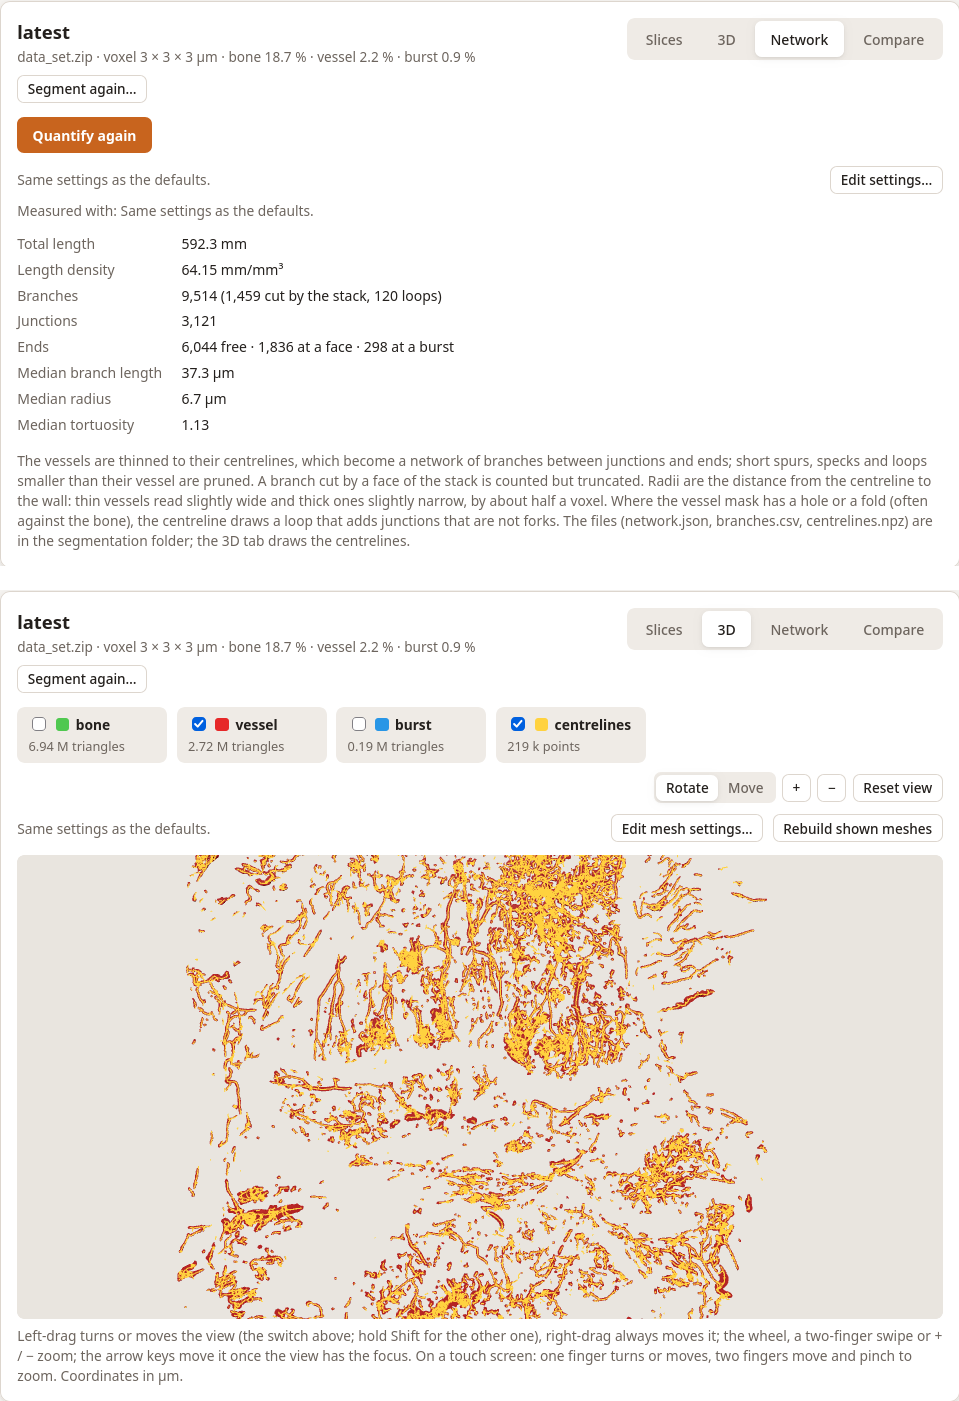
\includegraphics[width=0.95\linewidth]{../../screenshots/07-network.png}
  \caption{The page's Network tab after measuring the sample, and its centrelines drawn over the
    vessel mesh in the 3D view (zoomed in).}
  \label{fig:network-page}
\end{figure}
